\documentclass{beamer}

\mode<presentation>
{
  \usetheme{CambridgeUS}      % or try Darmstadt, Madrid, ...
  \usecolortheme{default} % or try albatross, beaver, crane, ...
  \usefonttheme{default}  % or try serif, structurebold, ...
  \setbeamertemplate{navigation symbols}{}
  \setbeamertemplate{caption}[numbered]
} 

\usepackage[english]{babel}
\usepackage[utf8x]{inputenc}
\usepackage{listings}
\usepackage[ampersand]{easylist}



\definecolor{KTI_green}{RGB}{150, 189, 13}
\definecolor{TU_red}{RGB}{255, 55, 81}
\definecolor{faint_gray}{RGB}{180, 180, 180}

\definecolor{syntax_green}{rgb}{0,0.6,0}
\definecolor{syntax_gray}{rgb}{0.9, 0.9, 0.9}
\definecolor{syntax_mauve}{rgb}{0.58,0,0.82}

\lstset{ 
  backgroundcolor=\color{syntax_gray},  % choose the background color
  basicstyle=\scriptsize\ttfamily,        		% size of fonts used for the code
  breaklines=false,                		% automatic line breaking only at whitespace
  captionpos=b,                    		% sets the caption-position to bottom
  commentstyle=\color{syntax_green},    % comment style
  escapeinside={\%*}{*)},          		% if you want to add LaTeX within your code
  keywordstyle=\color{blue},       		% keyword style
  stringstyle=\color{syntax_mauve},     % string literal style
  columns=fullflexible,
  frame=single,
  framesep=0.5cm,
  framexleftmargin=0.5cm,
  xleftmargin=0.5cm,
  framexrightmargin=0.5cm,
  xrightmargin=0.5cm,
  frame=tb,                 
    numbers=left,                    
    numbersep=15pt,  
  }
  
  
\newcommand{\logopython}{\raggedleft 
\includegraphics[height=0.5cm]{logo_python}\hspace{0.1cm}\\\raggedright}
\newcommand{\logopythonbottom}{\raggedleft\vspace{-0.8cm}
\includegraphics[height=0.5cm]{logo_python}\hspace*{0.05cm}\\\raggedright}

\title[BSP24 - Waschanlage]{Waschanlage}
\author{Dickbauer Y., Moser P., Perner M.}
\institute{PS Computergestützte Modellierung, WS 2016/17}
%\date{Date of Presentation}

\begin{document}

\begin{frame}
  \titlepage
\end{frame}

\begin{frame}{Outline}
  \tableofcontents
\end{frame}

\section{Aufgabenstellung}
\begin{frame}{Aufgabenstellung}
Bei der Planung einer Autowaschanlage muß der Besitzer entscheiden, wieviel Platz für
die wartenden Autos vorgesehen werden soll. Es wird geschätzt, dass die Kunden zufällig
(Poisson-Inputprozeß) mit einer mittleren Rate von einem Kunden alle 4 Minuten ankommen.
Ist der Warteplatz voll besetzt, würden ankommende Kunden mit ihren Fahrzeugen
wieder weiterfahren. \\~\\ Die Waschdauer ist in etwa exponentialveteilt mit einem Erwartungswert
von 3 Minuten. Vergleichen Sie den Erwartungswert des Anteils der potentiellen
Kunden, die wegen der fehlenden Wartemöglichkeit verloren gehen, wenn
\end{frame}

\begin{frame}{Aufgabenstellung}
\begin{enumerate}[(a)]
	\item kein Warteplatz
	\item zwei Warteplätze
	\item vier Warteplätze vorgesehen werden.
\end{enumerate}

\begin{itemize}
  \item Eingabe: -
  \item Output: Belegung der Warteplätze, Neuankünfte und Abfahrten
\end{itemize}
\end{frame}

\section{Flow Chart}
\begin{frame}{Flow Chart}
	\centering
  	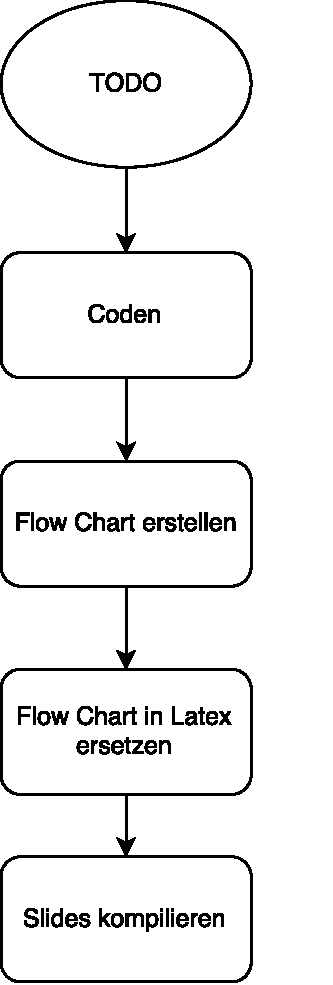
\includegraphics[scale=0.3]{FlowChartTodo.pdf}
\end{frame}

\subsection{Verwendete Funktionen}
%\begin{frame}[fragile]{Funktion loaded\_random\_choice(..)}
  \begin{itemize}
    \item Diese Funktion verlangt eine WSKL Liste als Eingabeparameter
    \item Gibt einen Index zurück, welcher 0 bis $\left\vert{probality\_list}\right\vert-1$ sein kann.
    \item Diese Indizes haben eine gewichtete WSKL, welche jeweils an der Position in der Eingabeliste steht
    \item Beispiel probility\_list := [ 0.9, 0.1 ]  $\Rightarrow$ mit p=90\% wird 0 zurückgegeben, p=10\% für 1
  \end{itemize}
  \begin{lstlisting}[language=python]
def loaded_random_choice(probability_list):
    n = len(probability_list)
    random_number = random.random()
    cum_p = 0
    for i in range(n):
        cum_p += probability_list[i]
        if cum_p > random_number:
            return i
    return None
\end{lstlisting}
\logopythonbottom
\end{frame}	

\section{Grafische Darstellung}
\begin{frame}{Ergebnis unserer Simulation}
	\centering
  	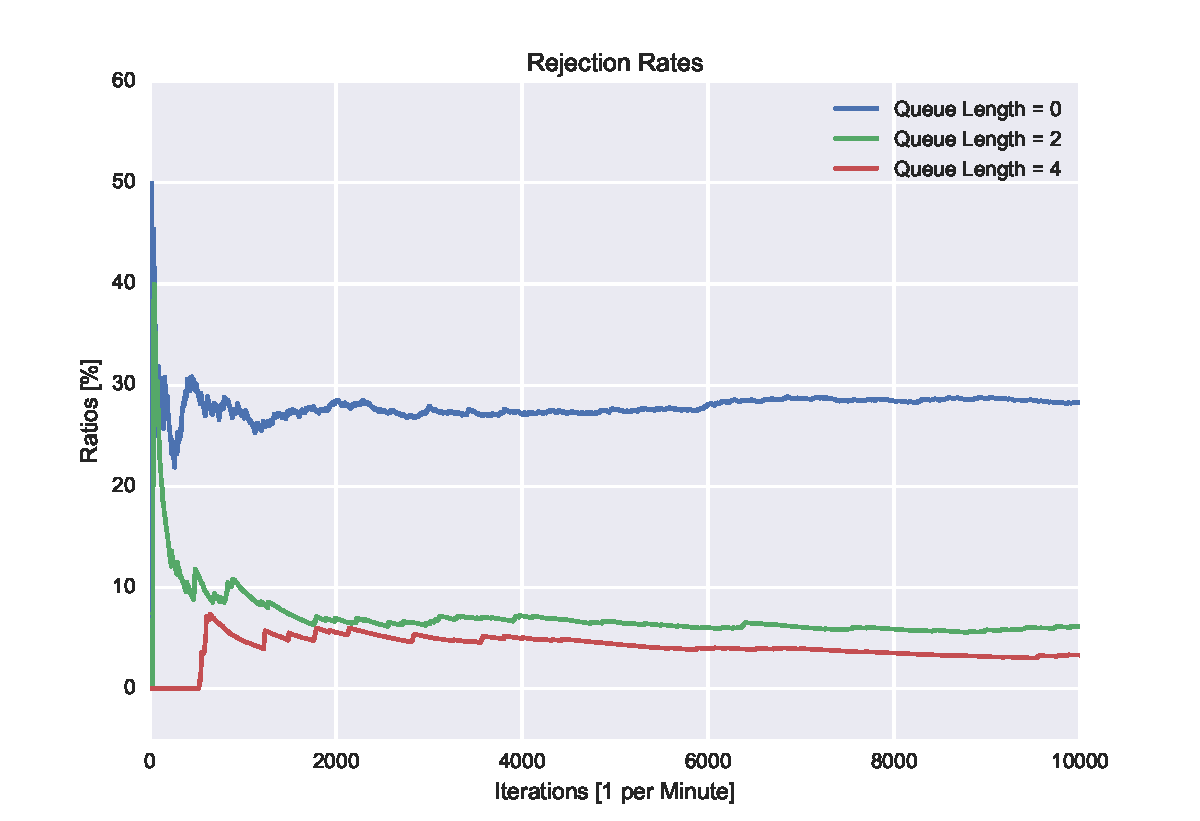
\includegraphics[scale=0.6]{BSP24_Plot.pdf}
\end{frame}

\end{document}
